%% -*- coding:utf-8 -*-
\chapter{Curry-Howard-Lambek correspondence}
\label{sec:curry_howard_lambek}
There is an interesting correspondence between computer programs and
mathematical proofs. Different types of logic correspond to different
computational models. This allows to build a theory of computation on
the base of math logic. First of all consider a category of proofs
\section{$\cat{Proof}$ category}
\begin{definition}[Proposition]
\label{def:proposition}
\textit{Proposition} is a statement that either true or false.
\end{definition}

There are 2 main propositions
\begin{definition}[True]
\label{def:true}
A true statement is one that is correct, either in all cases or at
least in the sample case \cite{bib:studycom:truefalse}. 
\end{definition}
and
\begin{definition}[False]
\label{def:false}
A false statement is one that is not correct \cite{bib:studycom:truefalse}. 
\end{definition}


\begin{example}[Proposition]
\label{ex:proposition}
There is an example of correct (true) proposition
\[
\forall n \in \mathbb{R}: n^2 \ge 0
\]

There is an example of incorrect (false) proposition
\[
\forall n \in \mathbb{C}: n^2 \ge 0,
\]
for instance $i \in \mathbb{C}$ gives $i^2 = -1$.

\end{example}

\begin{definition}[Implication]
\label{def:implication} \textit{An implication} is a
\mynameref{def:proposition} of the form $P \implies Q$ i.e. if $P$
then $Q$ \cite{bib:whatisaproof}.
\end{definition}

The main logical deduction rule is the following
\begin{definition}[Modus ponens]
\label{def:modusponens}
If $P$ is true and $P \implies Q$ is true then $Q$ is also true. The
rule is often written as \cite{bib:whatisaproof}
\[
\frac{
\begin{array}{c}
P \\
P \implies Q
\end{array}
}{Q}
\]
where if statements above the line are true then the statement below
the line is also true.
\end{definition}

\begin{definition}[Proof]
\label{def:proof}
\textit{Proof} is a verification \cite{bib:whatisaproof} of a
\mynameref{def:proposition} by a chain of logical deduction from a
base set of axioms.
\end{definition}

Propositions can be combined into new propositions via the following
logical operations
\begin{definition}[Conjunction]
\label{def:conjunction}
Conjunction or logical AND is the operation with following rules
  \begin{table}[H]
    \centering
    \caption{Conjunction}
    \label{tab:conjunction}
      \begin{tabular}{|l|l|l|}
        \hline
        $a$ & $b$ & $a \land b$ \\ \hline
        True & True & True \\ \hline
        True & False & False \\ \hline
        False & True & False \\ \hline
        False & False & False \\ \hline
      \end{tabular}
  \end{table}
\end{definition}
\begin{definition}[Disjunction]
\label{def:disjunction}
Conjunction or logical OR is the operation with following rules
  \begin{table}[H]
    \centering
    \caption{Disjunction}
    \label{tab:disjunction}
      \begin{tabular}{|l|l|l|}
        \hline
        $a$ & $b$ & $a \lor b$ \\ \hline
        True & True & True \\ \hline
        True & False & True \\ \hline
        False & True & True \\ \hline
        False & False & False \\ \hline
      \end{tabular}
  \end{table}
\end{definition}

Operations in Boolean logic follow the distributive law:
\begin{equation}
a \land ( b \lor c) = (a \land b) \lor (a \land c) 
\label{eq:distributive_law_boolean}
\end{equation}
i.e. the operation $\land$ corresponds to multiplication and $\lor$ to
sum. Therefore the $\cat{Proof}$ can be considered as a
\mynameref{def:distributive_category}. 

\begin{definition}[$\cat{Proof}$ category]
\label{def:proof_category}
The $\cat{Proof}$ category is a category where \mynameref{def:proposition}s are
\mynameref{def:object}s and \mynameref{def:proof}s are
\mynameref{def:morphism}s. I.e. proofs are used as connectors between
different propositions.
\end{definition}

Consider different objects and constructions of the proof (logic)
theory from the categorical point of view
\begin{example}[Initial object][$\cat{Proof}$]
\label{ex:proof_initial_object}
The \textit{false} statement can be considered as the initial object
because for any other statement exists only one proof from the false
statement to that one.
\end{example}

\begin{example}[Terminal object][$\cat{Proof}$]
\label{ex:proof_terminal_object}
The \textit{true} statement can be considered as the terminal object
\end{example}

\begin{example}[Product][$\cat{Proof}$]
\label{ex:proof_product}
\mynameref{def:conjunction} can be considered as
\mynameref{def:product} in \mynameref{def:proof_category}.
\end{example}

\begin{example}[Sum][$\cat{Proof}$]
\label{ex:proof_sum}
\mynameref{def:disjunction} can be considered as
\mynameref{def:sum} in \mynameref{def:proof_category}.
\end{example}

Thus we can declare the following correspondence (see
\cref{tab:curry_howard_lambek}) between logic 
proofs and \mynameref{def:cartesian_closed_category} and therefore
also between programming languages.
\begin{table}[H]
  \centering
  \caption{Relation between logic proofs and programming languages}
  \label{tab:curry_howard_lambek}
  \begin{adjustbox}{width=1\textwidth}
    \small
    \begin{tabular}{l|l|l}
      \toprule
      \mynameref{def:proof_category} & Programming language & 
      \mynameref{def:cartesian_closed_category}\\
      \midrule
      \mynameref{def:proposition}/\mynameref{def:implication} & Type &
      \mynameref{def:object} \\ 
      \mynameref{def:proof} & Function type & \mynameref{def:exponential} \\
      \mynameref{def:conjunction} & Product type & \mynameref{def:product} \\
      \mynameref{def:disjunction} & Sum type & \mynameref{def:sum} \\
      \mynameref{def:true} & unit type & \mynameref{def:terminal_object} \\
      \mynameref{def:false} & botom type & \mynameref{def:initial_object} \\
      \bottomrule
    \end{tabular}
  \end{adjustbox}
\end{table}


\section{Linear logic and Linear types}
Linear logic \cite{stanford:linear_logic} is one of refinements of
classical logic in the logic the \mynameref{def:implication} has been
modified. In the classical logic the both statements $P$ and $Q$ are
valid after implication $P \implies Q$. But in linear logic we have
another situation when the statement $P$ can be used only once and
become invalid after the usage. The situation then a resource can be used
only once is useful in different types of computations especially in
concurrency. TBD

\section{Quantum logic and quantum computation}

Different modifications of logic rules give us new computational
models. One of example is the quantum computations. The quantum logic
differs from Boolean one in the missing distributive law
\eqref{eq:distributive_law_boolean}. 

We can use the Heisenberg inequality to illustrate the violation of
the law. Consider a particle with 2 possible positions range and 1
possible momentum range. The event $P$ is that momentum has
range $\Delta p$. The event $Q_{1,2}$ is that position is in the
corresponding range $\Delta q_{1,2}$ (see \cref{fig:heisenberg}).

\begin{figure}[H]
  \centering
  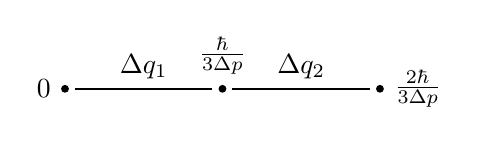
\begin{tikzpicture}[ele/.style={fill=black,circle,minimum
          width=.8pt,inner sep=1pt}]
      \node[ele,label=left:$0$] (a) at (0,0) {};
      \node[ele,label=above:$\frac{\hbar}{3 \Delta p}$] (b) at (2,0) {};
      \node[ele,label=right:$\frac{2 \hbar}{3 \Delta p}$] (c) at (4,0) {};
      \draw[-,thick,shorten <=2pt,shorten >=2pt] (a) to node[above]
           {$\Delta q_1$} (b);
      \draw[-,thick,shorten <=2pt,shorten >=2pt] (b) to node[above]
           {$\Delta q_2$} (c);  
  \end{tikzpicture}
  \caption{Heisenberg inequality. The event $P$ is that momentum has
    uncertainty $\Delta p$ Event $P \land Q_1$ is that particle's
    position is between $0$ and $\frac{\hbar}{3 \Delta p}$. Event
    $P \land Q_2$ is that particle's
    position is between $\frac{\hbar}{3 \Delta p}$ and
    $\frac{2\hbar}{3 \Delta p}$. Particle's position for event $P
    \land Q = (P \land Q_1)
    \lor (P \land Q_2)$ is between $0$ and $\frac{2\hbar}{3 \Delta p}$. The
    events $P \land Q_1$ and $P \land Q_2$ are forbidden by the Heisenberg
    inequality. From other side the event $P \land Q = (P \land Q_1)
    \lor (P \land Q_2)$ is possible}   
  \label{fig:heisenberg}
\end{figure}

Heisenberg inequality says
\[
\Delta p \Delta q_{1,2} \geq \frac{\hbar}{2}
\]
i.e. the following 2 events $P\land Q_{1,2}$ are not forbidden:
\[
\Delta p \Delta q_1 = \frac{\hbar}{3}
\]
and
\[
\Delta p \Delta q_2 = \frac{\hbar}{3}
\]
i.e.
\[
P \land Q_1 = P \land Q_2 = \mbox{False}
\]
from other side the event $P \land (Q_1 \lor Q_2)$ can be
$\mbox{True}$ as soon as
\[
\Delta p (\Delta q_1 + \Delta q_2) = \frac{2\hbar}{3} >
\frac{\hbar}{2}.
\]
Therefore we have distributive law
\eqref{eq:distributive_law_boolean} violation
\[
P \land (Q_1 \lor Q_2) \ne (P \land Q_1 ) \lor (P \land Q_2).
\]


